\documentclass[11pt,letterpaper,fleqn]{article}
\setlength{\parindent}{0 pt}
\usepackage[latin1]{inputenc}
\usepackage[T1]{fontenc}
\usepackage[spanish]{babel}
\usepackage{amsmath}
\usepackage{amsfonts}
\usepackage{amssymb}
\usepackage{graphicx}
\author{Rafael Hern�ndez S�nchez}
\title{Amplificadores de Clase B}
\begin{document}
		\pagestyle{plain}{
		\pagestyle{empty}
		
		\begin{center}
			\par\vspace{3cm}
			{
				\Huge\textbf{\textit{Universidad polit�cnica de la zona metropolitana de Guadalajara}}
			}
			\par\vspace{0.35cm}
			{
				\Large{\textbf{CARRERA:} Ingenieria en Mecatr�nica \\ \textbf{MATERIA:} Sistemas Electr�nicos de Interfaz \\ \textbf{MAESTRO:} Carlos Enrique Mor�n Garabito \\ \textbf{GRADO Y GRUPO:} 4-B}
			}
			\par\vspace{1cm}
			{
				\large\textbf{Tarea 5: Giro de un motor de corriente directa}
			}
			\par\vspace{1cm}
			{
				\large\textbf{Rafael Hern�ndez S�nchez \\ 15/10/19 \\}
			}
			
\includegraphics[scale=0.7]{UPZMG_Mecatr_nica}
			
			\par\vspace{3cm}
			
			
		\end{center}
		\clearpage
		\newpage
	}
\section{OBJETIVOS}
	\begin{itemize}
		\item Ver el funcionamiento del motor de corriente continua.
		\item Demostrar c�lculos y justificar su funcionalidad. 
	\end{itemize}
\section{MARCO TE�RICO}
	El motor de continua ha sido tradicionalmente muy utilizado por la facilidad de regulaci�n de su velocidad, simplemente variando la tensi�n aplicada. Tiene el inconveniente del mayor mantenimiento, cambio de escobillas, desgaste del colector, suciedad etc...
	\begin{center}
		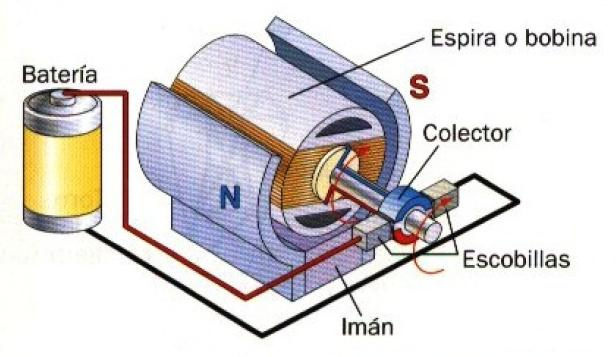
\includegraphics[scale=0.5]{1}
	\end{center}
	Para aplicaciones donde se necesita regulaci�n de velocidad se est� imponiendo el motor de alterna, por su mayor sencillez y por el abaratamiento de los variadores electr�nicos de frecuencia.
	En la pr�ctica hemos utilizado un peque�o motor de cc con excitaci�n mediante imanes permanentes, le hemos quitado las tapas y las hemos sustituido por placas de metacrilato, para que podamos ver su funcionamiento internamente.
	
\section{UTILIZACI�N}
	Su utilizaci�n en estos casos es importante el poder regular continuamente la velocidad del motor, adem�s, se utilizan en aquellos casos en los que es imprescindible utilizar corriente directa, como es el caso de motores accionados por pilas o bater�as. Este tipo de motores debe de tener en el rotor y el estator el mismo numero de polos y el mismo numero de carbones.\\
	
	\textbf{LOS MOTORES DE CORRIENTE DIRECTA PUEDEN SER DE TRES TIPOS:}\\
	\begin{itemize}
		\item SERIE
		\item PARALELO
		\item COMPOUND
	\end{itemize}
	\subsection{TIPO SERIE}
	Es un tipo de motor el�ctrico de corriente continua en el cual el devanado de campo (campo magn�tico principal) se conecta en serie con la armadura. Este devanado est� hecho con un alambre grueso porque tendr� que soportar la corriente total de la armadura.
	
	\begin{center}
		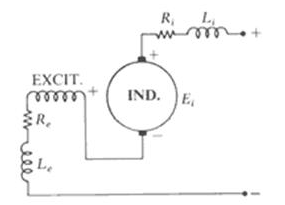
\includegraphics[scale=0.5]{2}
	\end{center}
	\subsection{TIPO PARALELO}
	Es un motor de corriente continua cuyo bobinado inductor principal est� conectado en derivaci�n con el circuito formado por los bobinados inducidos e inductor auxiliar.
	\begin{center}
		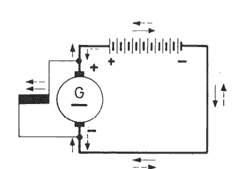
\includegraphics[scale=0.5]{3}
	\end{center}
	\subsection{TIPO COMPOUND}
	Es un motor de corriente continua cuya excitaci�n es originada por dos bobinados inductores independientes; uno dispuesto en serie con el bobinado inducido y otro conectado en derivaci�n con el circuito formado por los bobinados inducido, inductor serie e inductor auxiliar.
	\begin{center}
		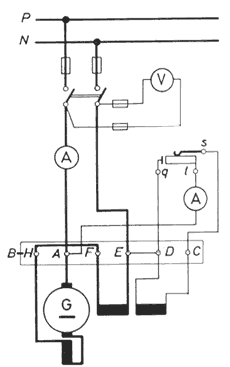
\includegraphics[scale=0.5]{4}
	\end{center}
\section{FUNCIONALIDAD}
Para controlar la velocidad y el sentido de giro de un motor de corriente continua. Depende y requiere de un circuito electr�nico especializado que realiza la regulaci�n de la velocidad mediante una t�cnica denominada PWM (Pulse Wide Modulation) y que consiste b�sicamente en variar la cantidad de tiempo que el motor recibe tensi�n. Si el motor recibe tensi�n. de forma constante, este gira a su m�xima velocidad y potencia.\\
Por lo que se hace, es aplicar la m�xima tensi�n del circuito pero no todo el tiempo, si no a pulsos, con lo que se consigue regular la velocidad manteniendo la potencia del motor.\\
Otro sistema de control consiste en regular la tensi�n. que se aplica al motor de forma que \underline{cuanto menos tensi�n, menos velocidad}. La pega de este sistema es que tambi�n pierde bastante potencia por lo que no es indicado la mayor�a de las veces.

\section{CONCLUCIONES}
\begin{itemize}
	\item En un motor el�ctrico de corriente continua es esencialmente una m�quina que convierte energ�a
	el�ctrica en movimiento o trabajo mec�nico.
	\item Los motores de CC son empleados para grandes potencias. Son motores industriales que
	necesitan una gran cantidad de corriente para el arranque.
	\item Los motores de CC llevan circuitos integrados para regular la toma de corriente de la l�nea y
	as� no generar bajones de intensidad de la corriente.
\end{itemize}
\section{BIBLIOGRAFIAS}
@online{monografias.com,
	author = { Sergio R. Tirado P.},
	title = {Motores de corriente directa (C.D.) },
	date = {7 de Mayo de 2015 },
	url = {https://www.monografias.com/trabajos74/motores-corriente-directa/motores-corriente-directa2.shtml},\\
}
@online{superrobotica.com,
	author = {Pablo Pompa},
	title = {Control de velocidad y giro para motor de corriente continua
	},
	date = {Febrero 2012},
	url = {http://www.superrobotica.com/conmotor.htm},
}
	
\end{document}